\documentclass[11pt]{article}

\input{../../preamble.tex}

\usepackage[letterpaper,margin=1in]{geometry}
\usepackage{amsmath,amssymb}
\usepackage{graphicx}
\usepackage{float}
\usepackage{array}
\usepackage{accents}
\usepackage{caption}

% Simple centered header like the PDF
\newcommand{\HandoutHeader}{
\begin{center}
{\Large University of British Columbia}\\[2pt]
{\large MECH 464/563 EECE 442/589 (Winter 2025): Introduction to Robotics}\\[2pt]
{\large HW Assignment 3, Forward Kinematics}
\end{center}
\vspace{0.8em}
}

\begin{document}
\HandoutHeader

Dominic Klukas, Student Number 64348378

Read Chapter 2, Forward Kinematics.

\vspace{1.0em}
\noindent \textbf{Exercise \#1.} \hfill (30 marks)

\noindent
Consider the manipulator below. Assign joint variables in a manner consistent with
the axes shown (positive angle by right hand rule), and coordinate systems
$\{\undertilde o_i, \underline C_i\}$, to all links, using the Denavit-Hartenberg convention. Complete the table of
Denavit Hartenberg parameters. Write, as a function of ${}^{i-1}\!T_i$, $i=0,\ldots,6$, the
coordinate transformation relating the coordinates ${}^{6}\!x$ in the gripper frame with the
coordinates ${}^{0}\!x$ in the base frame. You do not need to fill in the homogeneous matrices.

\begin{figure}[H]
  \centering
  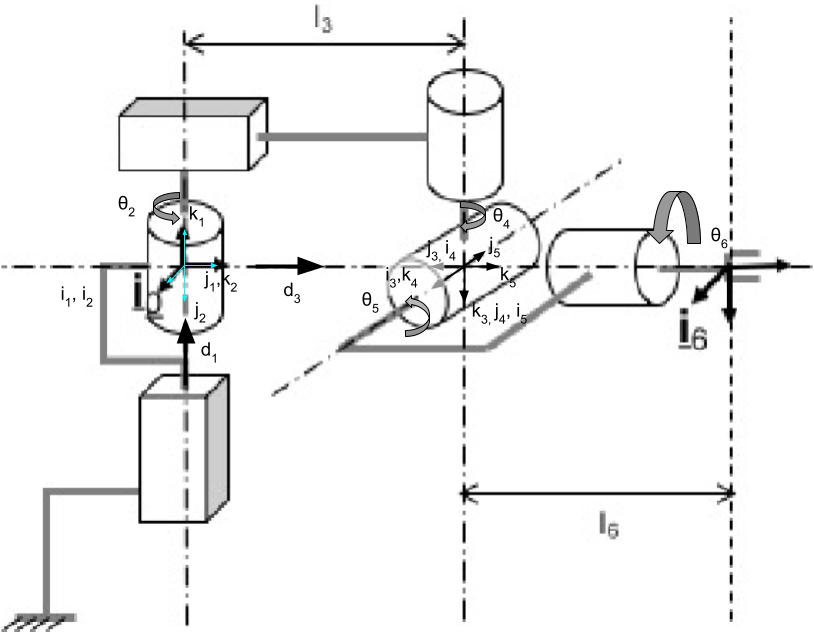
\includegraphics[width=0.55\textwidth]{figure1_cylindrical_robot.png}
  \caption{Cylindrical robot, with axes and co-ordinate systems added and labelled.}
\end{figure}

\vspace{0.5em}
\noindent\textbf{DH Parameters}\\[4pt]
% (Blank table for you to fill — you can change 6 to match your frame assignment)
\renewcommand{\arraystretch}{1.3}
\begin{center}
\begin{tabular}{|c|c|c|c|c|}
\hline
DH Parameter & $\theta_i$ & $d_i$ & $a_i$ & $\alpha_i$\\
\hline
Link 1 & 0 & $(d_1) $ & 0 & 0 \\
\hline
Link 2 & $(\theta_2)$ & 0 & 0 & -90 \\
\hline
Link 3 & 0 & $(d_3)$ & 0 & -90 \\
\hline
Link 4 & $(\theta_4) + 90 $ & 0 & 0 & $90$ \\
\hline
Link 5 & $(\theta_5) + 90$ & 0 & 0 & -90 \\
\hline
Link 6 & $-90$ & $l_6$ & 0 & 0 \\
\hline
\end{tabular}
\end{center}

\vspace{0.8em}
\noindent\textbf{Transformation chain (Exercise \#1)}\\[4pt]
\[
{}^{0}\!x \;=\; {}^{0}\!T_{6}\,{}^{6}\!x,
\qquad
{}^{0}\!T_{6} \;=\; {}^{0}\!T_{1}\,{}^{1}\!T_{2}\,{}^{2}\!T_{3}\,{}^{3}\!T_{4}\,{}^{4}\!T_{5}\,{}^{5}\!T_{6}.
\]

\vspace{1.2em}
\noindent \textbf{Exercise \# 2:} \hfill (30 marks for (a) and (b), 40 marks for (c))

\noindent
The Puma 560 shown in Figure 2 has a reach of approximately 0.92m, and a payload
capacity of 2.3kg. It was widely used for medium-to-lightweight assembly, welding,
materials handling, packaging and inspection applications.

\noindent
Using the schematic of Figure 3, do the following:

\begin{figure}[H]
  \centering
  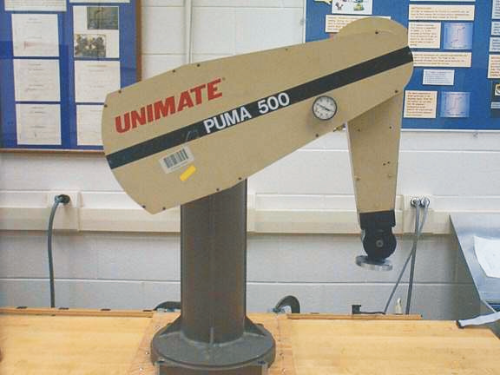
\includegraphics[width=0.70\textwidth]{figure2_puma_photo.png}
  \caption{Photo of a 500 series Puma robot.}
\end{figure}

\noindent
(a) Directly on the schematic, assign coordinate frames by means of the Denavit-Hartenberg
convention. Assume $C_0$ and $C_6$ are as illustrated in the ``home'' position. Fill in Table 1
the values of the DH-parameters. For each joint, consider the positive rotation to be in the
right-handed sense.


See Figure 3 for the co-ordinate frame placement.

\vspace{0.6em}
\noindent\textbf{Table 1: DH Parameters for the Puma 560}

\renewcommand{\arraystretch}{1.35}
\begin{center}
\begin{tabular}{|>{\raggedright\arraybackslash}p{1.8cm}|c|c|c|c|}
\hline
DH Parameter & $\theta_i$ (deg) & $d_i$ (mm) & $a_i$ (mm) & $\alpha_i$ (deg)\\
\hline
Link 1 & $(\theta_1)$ & 0 & 0 & $-90$ \\
\hline
Link 2 & $(\theta_2)$ & 0  & 430.0 & 180 \\
\hline
Link 3 & $(\theta_3) + 90$ & -149.1 & 20.3 & 90 \\
\hline
Link 4 & $(\theta_4)$ & 435.0 & 0 & 90 \\
\hline
Link 5 & $(\theta_5)$ & 0 & 0 & -90 \\
\hline
Link 6 & $(\theta_6)$ & 60.0 & 0 & 0 \\
\hline
\end{tabular}
\end{center}

\noindent
(b) Compose a chain of transformations that will give you the relationship between the base
coordinate system $\{o_0, C_0\}$ and the end-effector coordinate system $\{o_6, C_6\}$.
Use the same notation we have used for the Stanford manipulator (slides or p.7 Forward
Kinematics notes).

\vspace{0.6em}
\noindent\textbf{Transformation chain}\\[4pt]
In the notation of page 7 in the notes:
\begin{align*}
    \begin{bmatrix} \underline C_{6} & \undertilde o_6 \\ 0^T & 1 \end{bmatrix} &= \begin{bmatrix} \underline C_{6} & \undertilde o_6 \\ 0^T & 1 \end{bmatrix} {}^{0}T_1 (\theta_1) {}^{1}T_2 (\theta_2) {}^{2}T_3 (\theta_3) {}^{3}T_4 (\theta_4) {}^{4}T_5 (\theta_5) {}^{5}T_6 (\theta_6) \\
                                     &= \begin{bmatrix} \underline C_{6} & \undertilde o_6 \\ 0^T & 1 \end{bmatrix} {}^{0} T_6 (\theta_1, \theta_2, \theta_3, \theta_4, \theta_5, \theta_6)
.\end{align*}

\noindent
(c) Write a MATLAB m-file which allows the user to input the 6 joint angles (in degrees),
and outputs both the resulting homogenous transformation matrix (relating the base and end
effector coordinate systems). You will need to do direct kinematics from DH parameters for
other robots, so you might as well include a function that takes an array of DH parameters
and produces the gripper-to-base homogeneous transformation ${}^{0}\!T_{n}$.
Demonstrate this (e.g., use diary) by computing the end-effector transformations for the
following joint vector sets:
\[
q_A=[0;0;0;0;0;0]^T,\quad
q_B=[0;0;-90;0;0;180]^T,\quad
q_C=[45;-45;45;0;-30;90]^T.
\]

The computed end-effector transformations:
\begin{align*}
    T_A &=
\begin{bmatrix}
    0&  0  &  1.0000 &  925.0000\\
    0& -1.0000 &   0  & 149.1000\\
    1.0000&0&0&20.3000\\
    0&0&0&1.0000
\end{bmatrix}\\
    T_B &=
\begin{bmatrix}
-1.0000&        0 &       0 &450.3000\\
         0 &  1.0000 &       0 &149.1000\\
         0       & 0  &-1.0000&-495.0000\\
         0       & 0       & 0 &  1.0000
\end{bmatrix}\\
    T_C &=
\begin{bmatrix}
 0.7071  & 0.6124 & -0.3536 & 74.0029\\
   -0.7071  & 0.6124 & -0.3536 &284.8621\\
         0  & 0.5000 &  0.8660 &791.0174\\
         0  &      0 &       0 &  1.0000
\end{bmatrix} 
.\end{align*}

\begin{figure}[H]
  \centering
  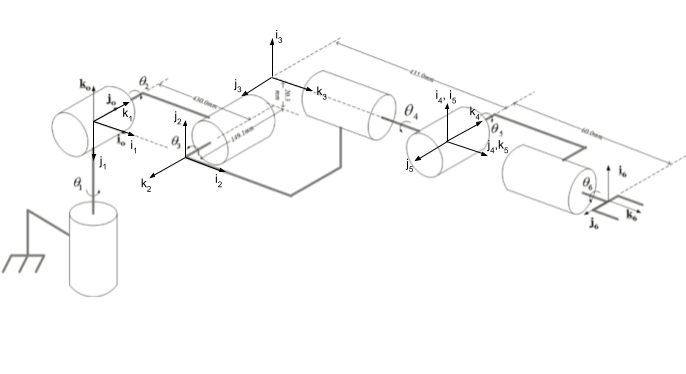
\includegraphics[width=0.85\textwidth]{figure3_puma_schematic.png}
  \caption{The Puma 560 robot schematic with co-ordinate frames (not to scale).}
\end{figure}


Matlab function:
\begin{verbatim}
function T = dh_fk(DH, q)
% Computes the transformation matrix given DH parameters (6*4 matrix) where
% angles are in degrees.
% parameters q = 1*n array with revolute joint angles (assumes only
% revolute joints), also in degrees.
    n = size(DH, 1); % Number of joints
    T = eye(4); % Initialize transformation matrix as identity
    for i = 1:n
        theta = (DH(i, 1) + q(i));
        d = DH(i, 2);
        a = DH(i, 3);
        alpha = DH(i, 4);
        % Formula for transformation given 4 DH parameters
        Tthet = eye(4);
        Tthet(1:3, 1:3) = rotz(theta);
        Td = eye(4);
        Td(3, 4) = d;
        Ta = eye(4);
        Ta(1, 4) = a;
        Talph = eye(4);
        Talph(1:3, 1:3) = rotx(alpha);
        T = T*Tthet * Td * Ta * Talph;
    end
end 
\end{verbatim}

\end{document}

